% Copyright (C) Huawei Technologies Co., Ltd. 2024. All rights reserved.
% SPDX-License-Identifier: MIT
\begin{frame}[fragile]{Weak Memory Consistency Models (WMMs)}
	\begin{columns}[c]
		\column{.5\textwidth}{%
			\centering
			\begin{itemize}\setlength{\itemindent}{-1em}
				\item Modern architectures becoming popular\\ \eg, {Arm}, {RISC-V}\\[8pt]
				\item<7-> {\bf Aggressive reorderings} to improve sequential performance\\[8pt]
					%\item<7-> Nightmare for concurrent code!
				\item<7-> {\bf Much higher non-determinisim};\\
					even harder to test!\\[8pt]
				\item<7-> Careful use of {\bf memory barriers}\\ (neither too many, nor too few)
			\end{itemize}
			%\resizebox{.5\textwidth}{!}{\input{figs/store-buffering}}
			%\uncover<7->{\hspace{-10mm}\resizebox{.9\textwidth}{!}{% Copyright (C) Huawei Technologies Co., Ltd. 2024. All rights reserved.
% SPDX-License-Identifier: MIT
\begin{tikzpicture}[
    a/.style = {->, thick},
    j/.style = {fill=white, font=\scriptsize\bf},
    b/.style = {rounded corners, align=left}, %, text width = 7mm},
    i/.style = {b},
    t/.style = {b, fill=light gray},
    c/.style = {b, fill=light red, text width=34mm},
    ]
\coordinate (x);
\node[i, above=10mm of x] (a) {\verb|msg = 0; ready = false;|};
\node[t, left=5mm of x] (b1) {\verb|msg = 42;|\\ \verb|ready = true;|};
\node[t, right=0mm of x] (b2) {\verb|while(!ready) {}|\\{\verb|assert(msg == 42);|}};
%\node[c, below=of x] (c) {\verb+assert(a != 0 || b != 0);+};
%\draw[a]  (a) -- (b1);
%\draw[a]  (a) -- (b2);
%\draw[a]  (b1) -- (c);
%\draw[a]  (b2) -- (c);
%\node[j, below=1mm of a] {{\tt pthread_create}};
%\node[j, above=1mm of c] {{\tt pthread_join}};
\node[j, above=0 of a] {Init};
\node[j, fill=none, above=0 of b1] (t1) {Thread 1};
\node[j, fill=none, above=0 of b2] (t2) {Thread 2};
\node[text=HuaweiRed, right=-2mm of b2.south east, yshift=2.5mm] {\xmark};

%\draw[a]  (a) -- (t1);
%\draw[a]  (a) -- (t2);
\draw<1->[<->, very thick, HuaweiRed] (b1.170) to [out=180, in = 90]
node[midway, left=1mm, align=center, font=\scriptsize] {WMM\\reorder}
+(-4mm, -2mm) to [out = -90, in = 180] (b1.190);
\end{tikzpicture}
}}
		}\column{.5\textwidth}{%
			\centering
			%\only<-7>{\resizebox{!}{.8\textheight}{%
			\only<-7>{\resizebox{.8\textwidth}{!}{%
					\begin{tikzpicture}[cut/.style={draw, very thick,fill=white}]
						\draw[draw=none, dotted, use as bounding box] (0cm,-48mm) rectangle (8cm, 48mm);
						\node<2-7>[cut] at (35mm, 25mm) (a1) {
\includegraphics[width=7cm]{figs/arm-huawei}};
						\node<3-7>[cut, below right=13mm and -1cm of a1.north] (a2) {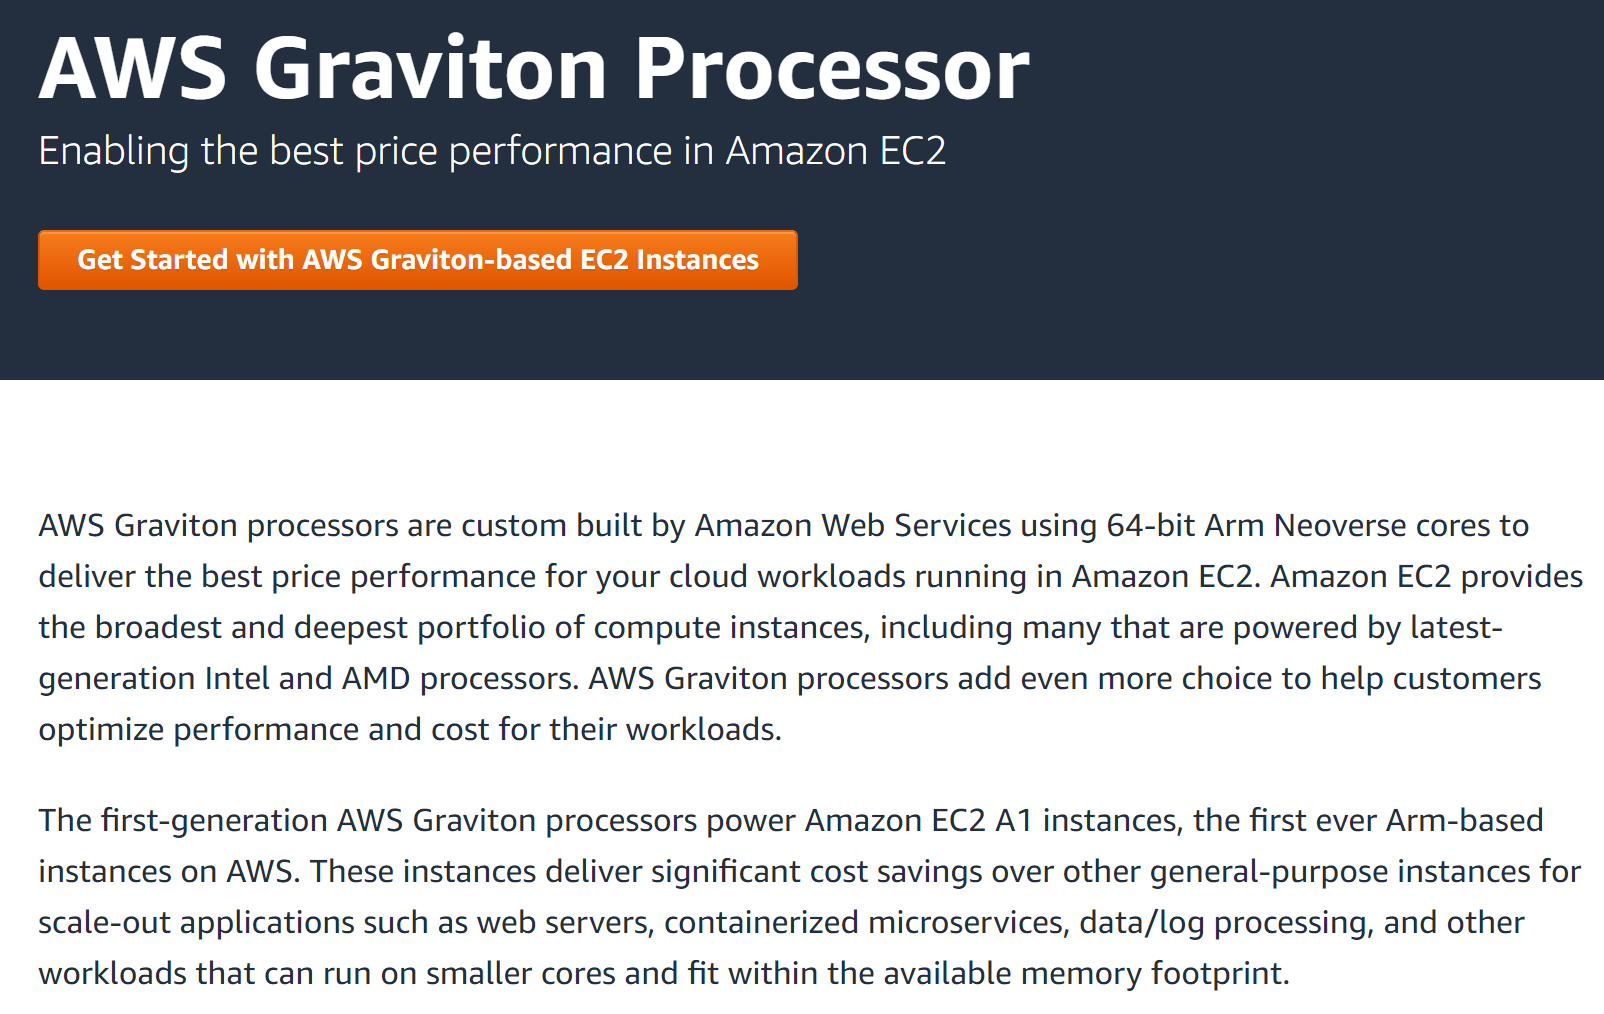
\includegraphics[width=7cm]{figs/arm-amazon}};
						\node<4-7>[cut, below left=18mm and -2mm of a2.north] (a3) {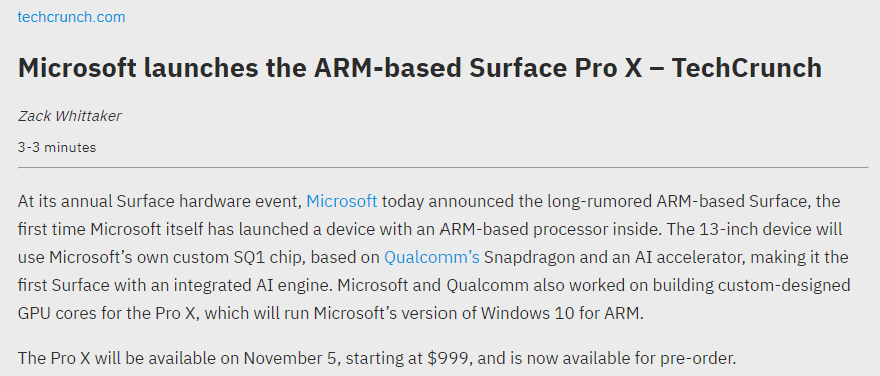
\includegraphics[width=7cm]{figs/arm-microsoft}};
						\node<5-7>[cut, below right=15mm and -28mm of a2.north] (a3) {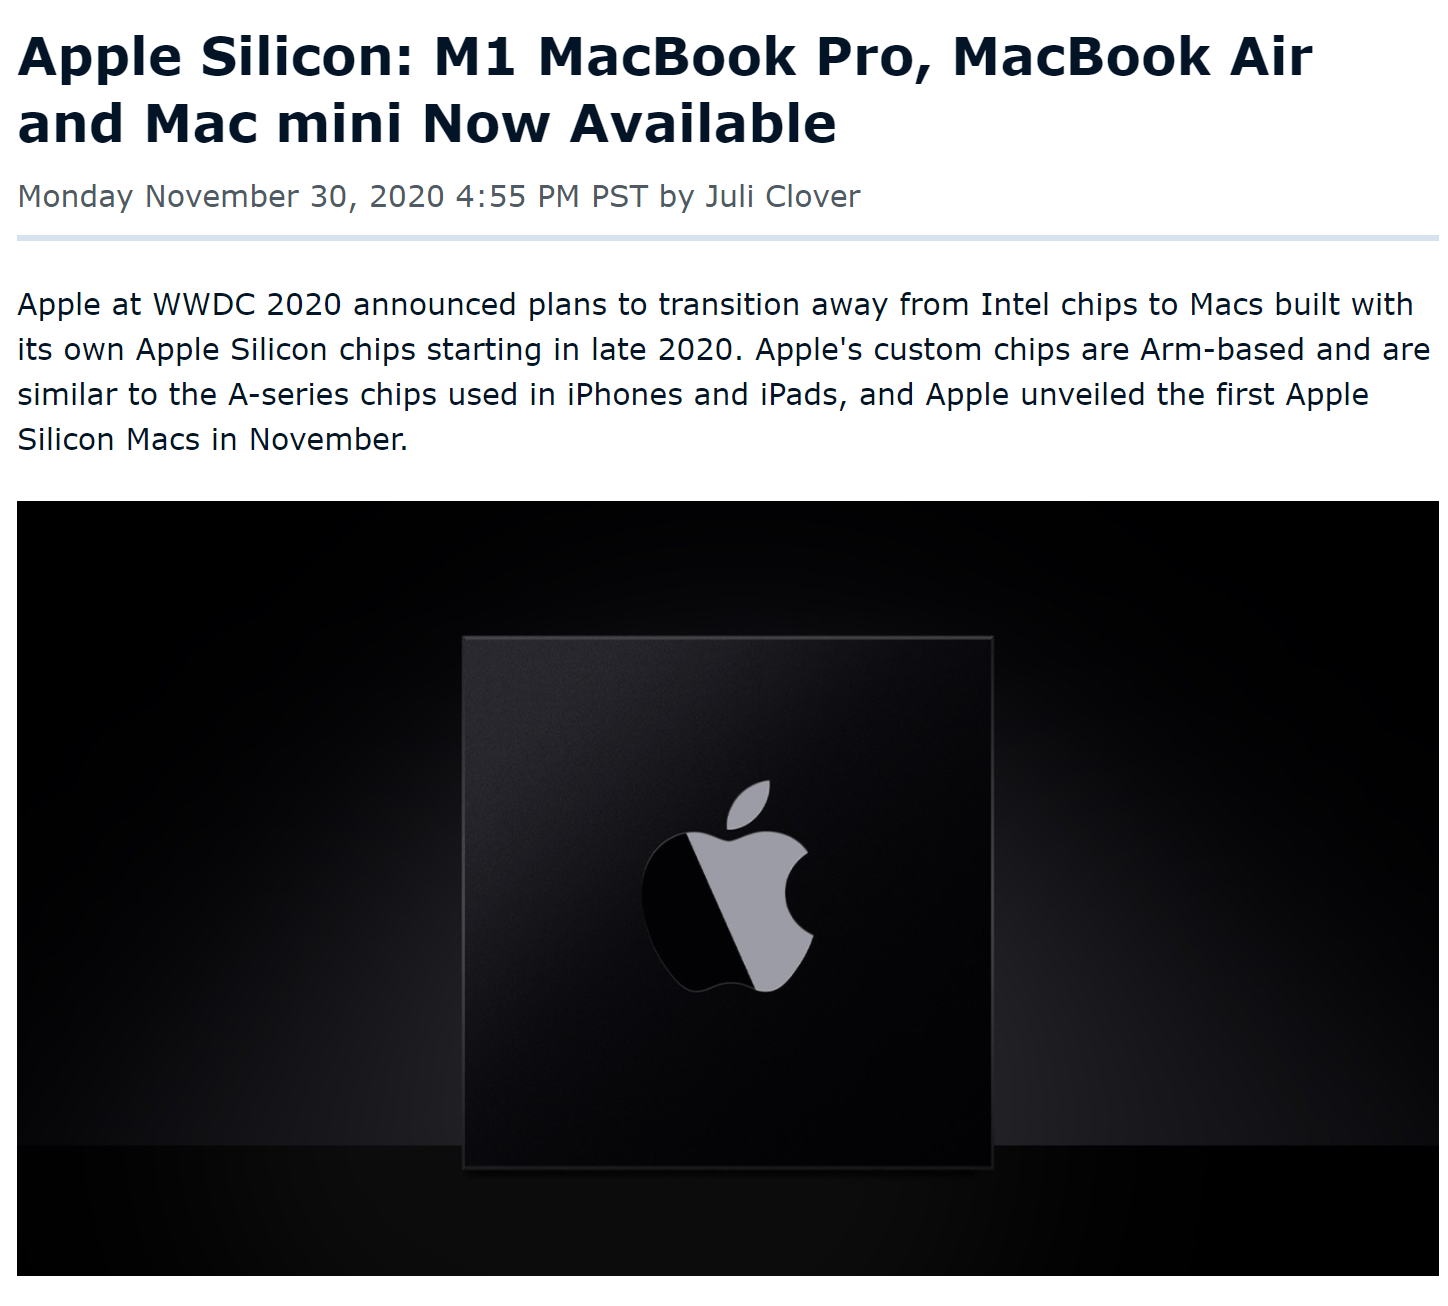
\includegraphics[width=7cm]{figs/arm-apple}};
						\node<6-7>[cut, below right=35mm and -8cm of a2.north] (a4) {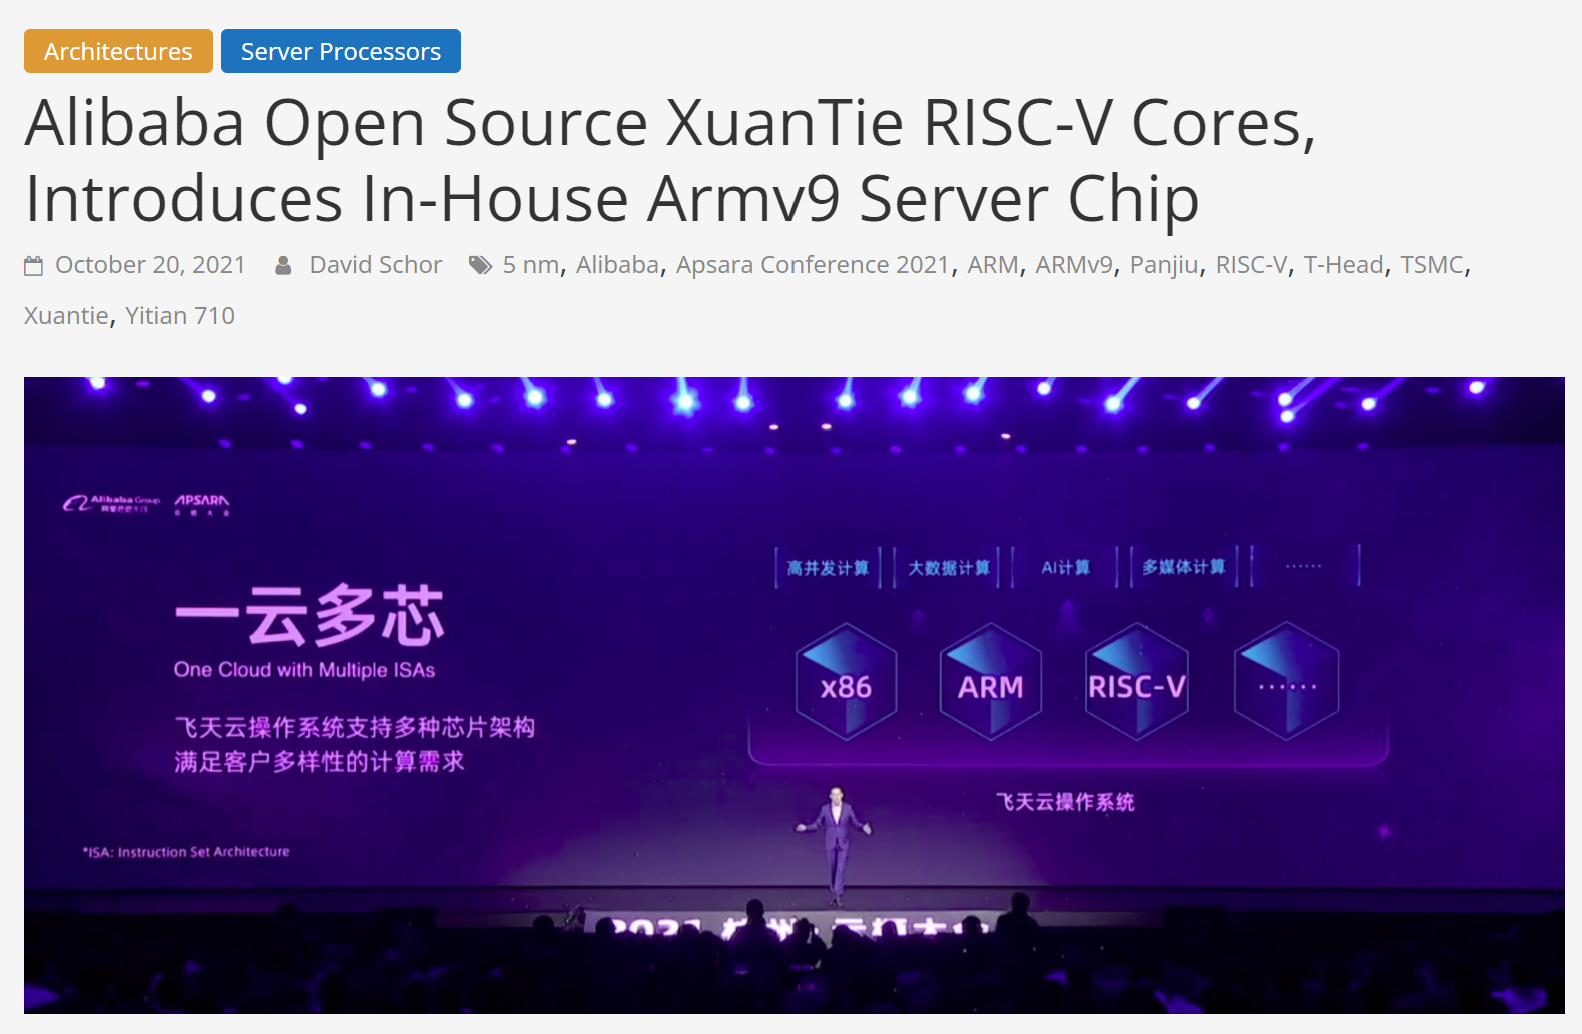
\includegraphics[width=7cm]{figs/arm-alibaba.png}};
					\end{tikzpicture}}}%
		}
	\end{columns}
\end{frame}
